% class
\documentclass[ngerman]{scrartcl}

% input preamble
\input{../../shared_preamble.tex}

% biblatex
\addbibresource{advanced_microscopy.bib}


% manual header
\ihead{Advanced Microscopy}  % inner (left) head
\chead{\textsc{Wachmann} Elias (12004232)\\\textsc{Zach} Andreas (12004790)}  % center head
\ohead{31.03.2023}  % outer (right) head



\begin{document}

\begin{titlepage}
    \centering
    \includegraphics[width=0.5\textwidth]{../../99_Misc/Logo_KF.pdf}\par\vspace{0.8cm}
    {\scshape\LARGE{Karl-Franzens-Universität Graz}\par}
    {\scshape\LARGE{Institut für Physik}\par}
    \vspace{1cm}
    {\scshape\Large{23S PHY.L02UB Fortgeschrittenenpraktikum 2}\par}
    678 Bachelorstudium Physik, UG2002/2021W\par
    \vspace{1.5cm}
    {\huge\bfseries IV. Advanced Microscopy\par}
    \vspace{2cm}
    \begin{table}[H]
        \centering
        \begin{tabular}{c c c}
            \Large \textsc{Wachmann} Elias &  & \Large \textsc{Zach} Andreas \\
            \Large 12004232                &  & \Large 12004790              \\
            \multicolumn{3}{c}{Gruppe 12}
        \end{tabular}
    \end{table}
    \vfill
    \Large Betreut von\par
    % Assoz. Prof. Mag. Dr.rer.nat. Georg \textsc{Koller}
    Dr. Georg \textsc{Koller}
    \vfill
    {\large 31.03.2023\par}
\end{titlepage}

\clearpage
\tableofcontents
\newpage

\section[Aufgabenstellung]{Aufgabenstellung \cite{ref:angabe}}
\label{sec:aufgabenstellung}

Der vorliegende Laborversuch teilt sich in Unterversuche, welche wie folgt gegeben sind:

\begin{itemize}
    \item Abbildung durch eine Sammellinse
          \begin{itemize}
              \item Mittels Lupeneffekt
              \item Mittels Abbildungsgleichung
              \item Mittels Bessel-Verfahren
          \end{itemize}
    \item Das 1-Linsen-Mikroskop nach \textsc{van Leeuwenhoek}
          \begin{itemize}
              \item Aufbau des Mikroskops
              \item Qualitatives Betrachten von Objekten
              \item Bestimmung der effektiven Fokuslänge
              \item Bestimmung des Brechungsindex, ab welchem der Fokuspunkt innerhalb der Kugellinse liegt
          \end{itemize}
    \item Hellfeld-Transmissionsmikroskop
          \begin{itemize}
              \item Aufbau des Mikroskops und Einrichtung
              \item Aberrationen
                    \begin{itemize}
                        \item Linsenorientierung (Objektiv) und sphärische Aberration
                        \item Kohärenz der Beleuchtung
                        \item Wellenlängenabhängigkeit und chromatische Aberration
                    \end{itemize}
              \item Charakteristika des Mikroskops
                    \begin{itemize}
                        \item Gesamtvergrößerung
                        \item Auflösungsvermögen
                    \end{itemize}
          \end{itemize}
    \item Dunkelfeldmikroskop
          \begin{itemize}
              \item Aufbau des Mikroskops und Einrichtung
              \item Vergleich mit dem Hellfeld-Transmissionsmikroskop
          \end{itemize}
\end{itemize}


\section[Voraussetzungen und Grundlagen]{Voraussetzungen und Grundlagen \cite{ref:angabe}}
\label{sec:voraussetzungen_grundlagen}

\subsection{Abbildung durch eine Sammellinse}
\label{subsec:abbildung_sammellinse_Grundlagen}

Für den vorliegenden Versuch soll die Fokuslänge/Brennweite $f$ der Sammellinse bestimmt werden. Dazu werden drei verschiedene Methoden angewendet:

\paragraph{1.}
Zuerst soll die Brennweite über den \enquote{Lupeneffekt} bestimmt werden, indem ein sehr weit entferntes Objekt (Abstand zur Linse $\gg f$) scharf abgebildet wird.

\paragraph{2.} Die Brennweite kann auch aus der Linsengleichung
%
\begin{equation}
    \label{eq:linsengleichung}
    \frac{1}{f} = \frac{1}{g} + \frac{1}{b}
\end{equation}
%
experimentell bestimmt werden ($g$ Gegenstandsweite, $b$ Bildweite, $G$ Genestandsgröße, $B$ Bildgröße; siehe auch \autoref{fig:sammellinse}). Als Beleuchtung wird eine Halogenlampe und als Objekte zur Verfügung
stehende Proben verwendet. Die entsprechenden Abstände $b$ und $g$ werden mittels Lineal und die Größen $B$ und $G$ mittels Kamera gemessen.
%
\begin{figure}[H]
    \centering
    \begin{samepage}
        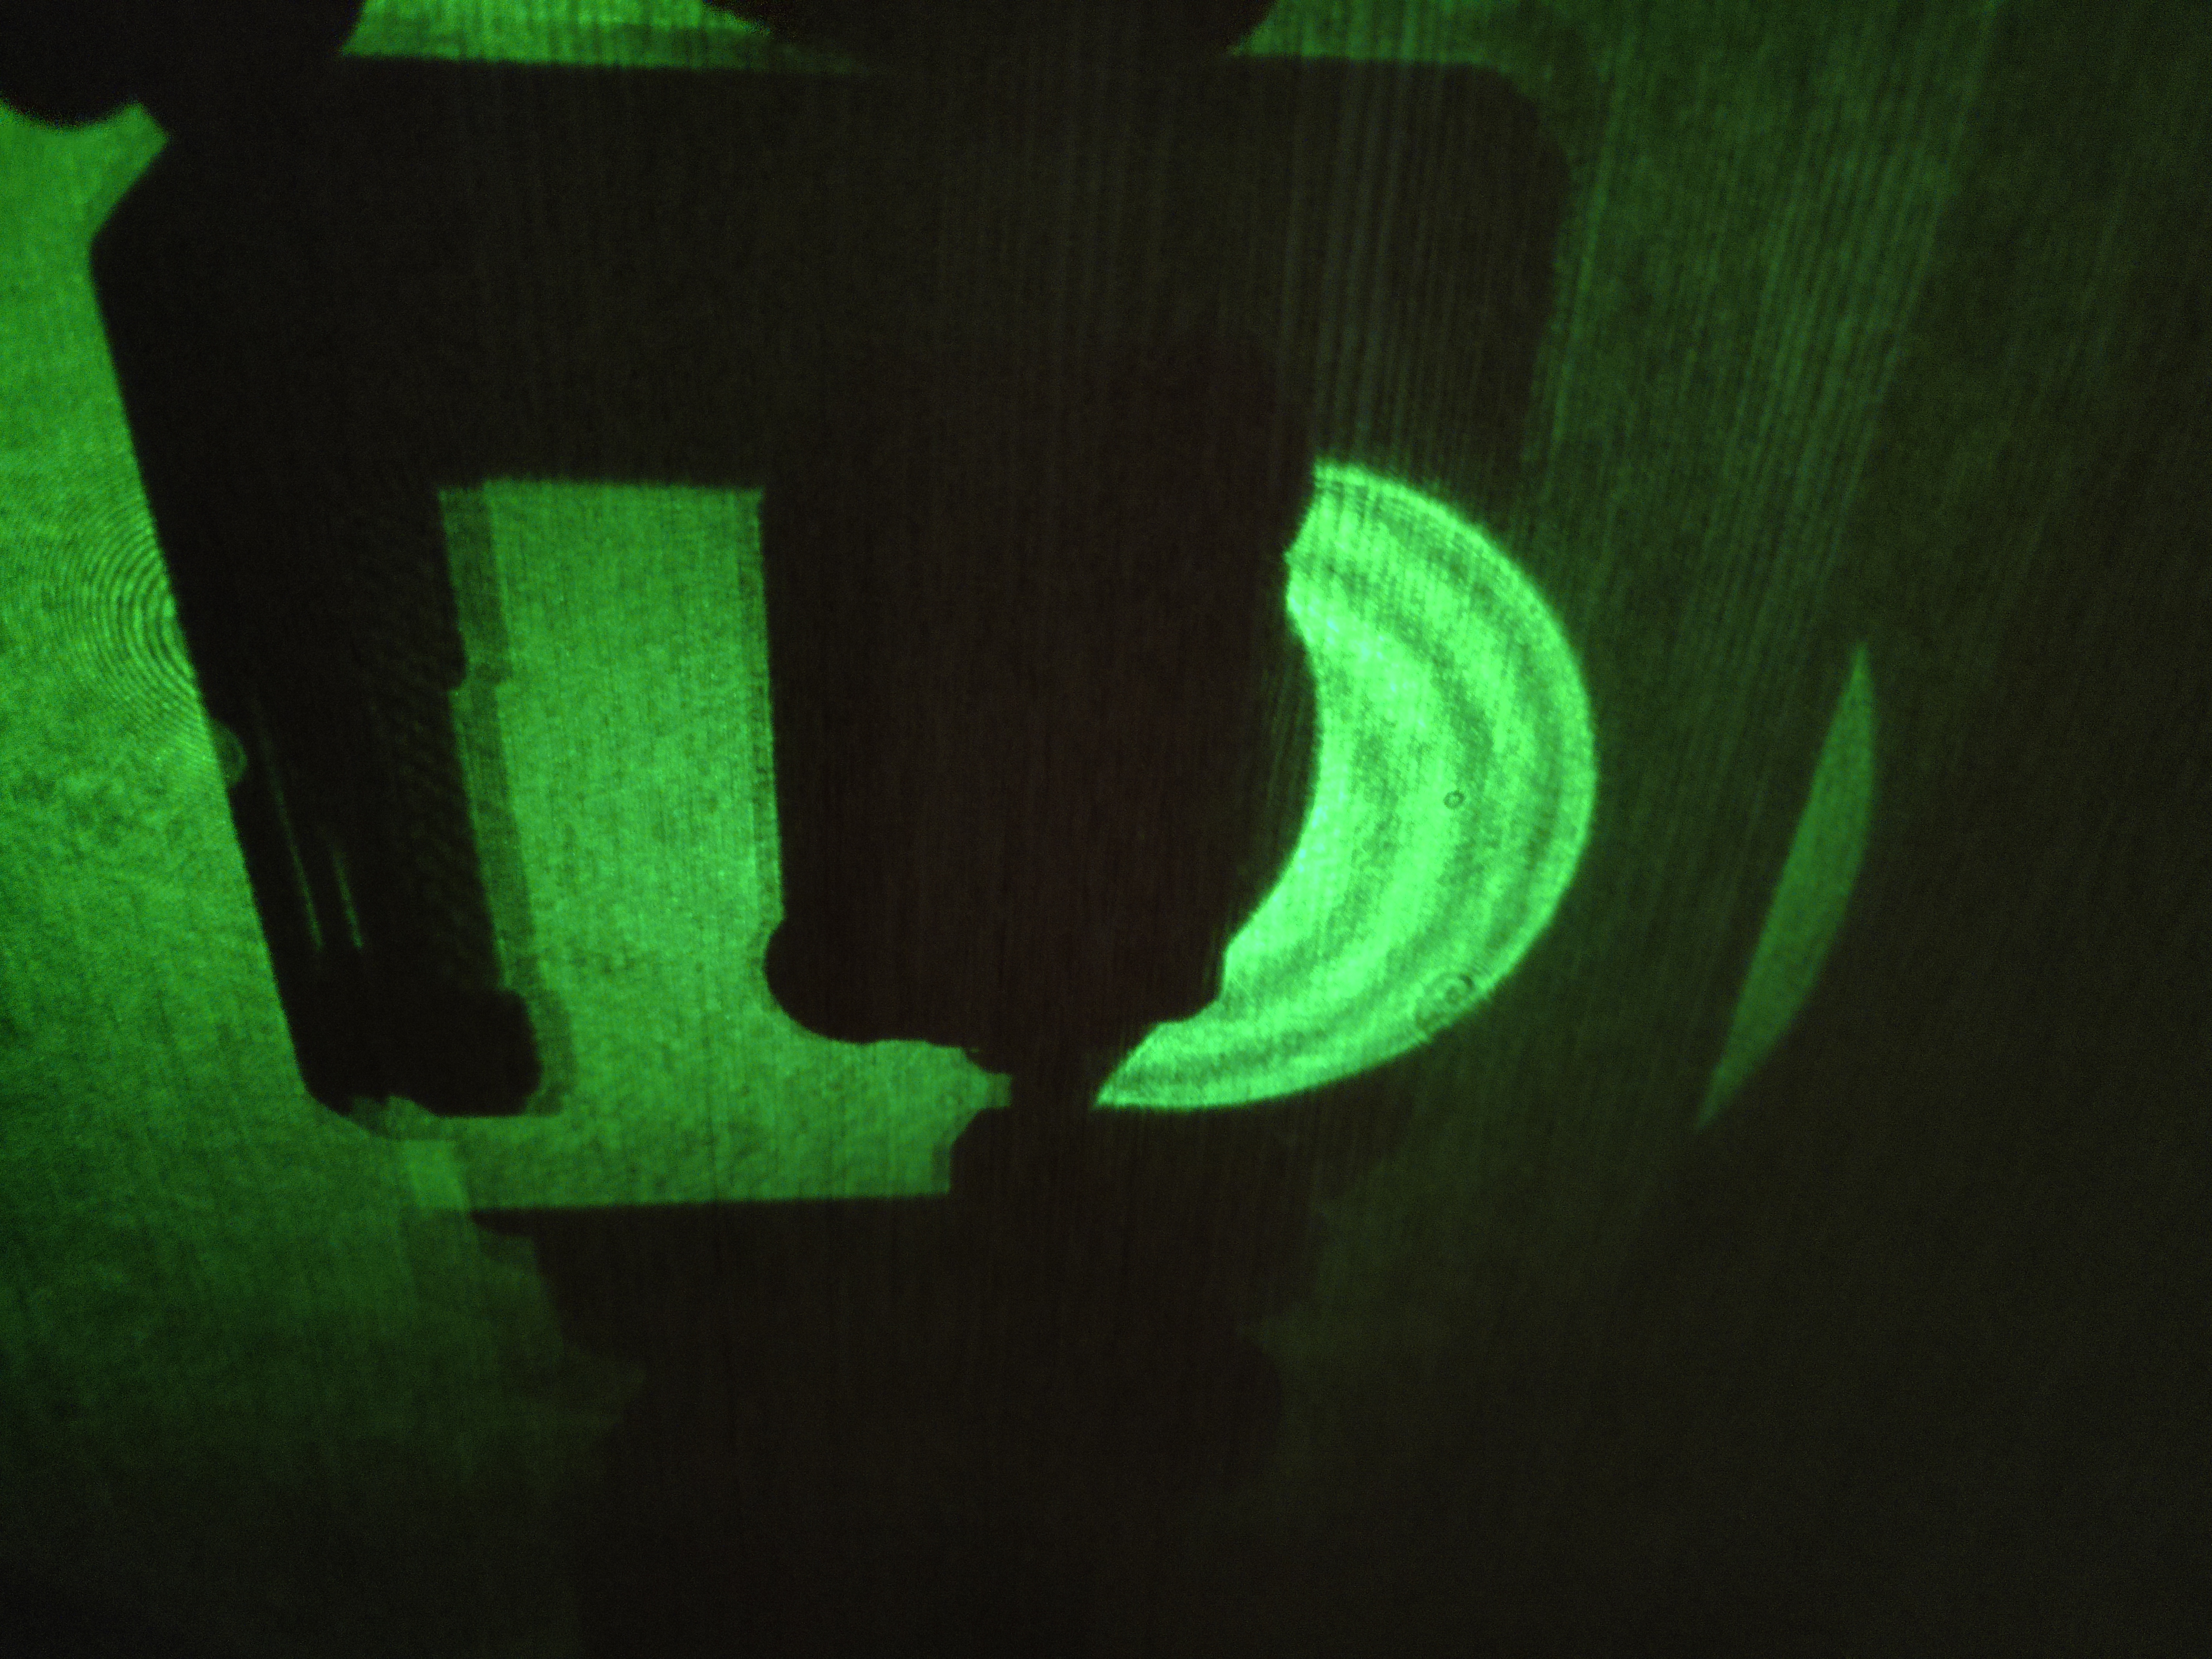
\includegraphics[width=\linewidth]{fig/Sammellinse.png}
        \caption[Strahlengang einer Sammellinse]{Strahlengang zur Abbildung mithilfe einer einzelnen Sammellinse zusammen mit den wichtigsten Parametern. Konstruktion eines Bildes: Parallelstrahl wird zum Brennstrahl (grün) und Brennstrahl zum Parallelstrahl (gelb). Schnittpunkt mit Mittelpunktstrahl (blau) definiert Bildweite $b$ und Bildgröße $B$.}
        \label{fig:sammellinse}
    \end{samepage}
\end{figure}

\paragraph{3.}
Zuletzt wird zur Bestimmung der Brennweite das sogenannte \textit{Bessel-Verfahren} oder \textit{Bessel'sches Verschiebeverfahren} verwendet. Hierzu wird wieder ein Gegenstand im Versuchsaufbau mit der Linse scharf abgebildet (auf Mattscheibe oder Kamera). Bei festem Abstand $l$ von Gegenstand und Position des scharf abgebildeten Bildes ($l = b + g = \text{const.}$) lässt sich eine zweite Position der Linse finden, für die eine scharfe Abbildung möglich ist ($l = b_1 + g_1 = b_2 + g_2$). Aus dem Gesamtabstand $l$ und den Abstand $w$ zwischen beiden Linsenpositionen lässt sich letztendlich die Brennweite $f$ bestimmen. Dazu gilt folgende Gleichung unter der Annahme dünner Linsen:
%
\begin{equation}
    \label{eq:bessel}
    f = \frac{l^2 - w^2}{4 l}
\end{equation}


\subsection{Das 1-Linsen-Mikroskop nach van Leeuwenhoek}
\label{subsec:1_linsen_mikroskop_Grundlagen}

Antonie van Leeuwenhoek (1632-1723) gilt als einer der ersten erfolgreichen Konstrukteure von einfachen Mikroskopen mit (bis zu seiner Zeit) unerreicht hohen Vergrößerungen und beeindruckender Bildqualität. Durch die hohe Qualität der Linsen und die clevere Konstruktion seiner 1-Linsen-Mikroskope, die teils eher an sehr starke Lupen erinnern, konnte er Auflösungen im Mikrometerbereich erreichen und Mikroorganismen abbilden (und diese dabei auch erstmals nachweisen!). Aufgrund dieser Erfolge wird er auch als Vater der Mikrobakteriologie bzw. Mikrobiologie bezeichnet. Um die genauen Methoden seiner mikroskopischen Messungen ranken sich viele Mythen und Interpretationsversuche, da er die Details bzgl. der Messprozedur sowie der genauen Vorgehensweise zur Herstellung von Linsen, das Kernstück seiner Geräte, stets geheim hielt.
%
\begin{figure}[H]
    \centering
    \begin{samepage}
        \includegraphics[width=\linewidth]{fig/Leeuwenhoek.png}
        \caption[Aufbau eines van Leeuwenhoek Mikroskops]{(a) Bild eines einfachen Mikroskops von van Leeuwenhoek mit Beschreibung der einzelnen Bauteile. (b) Einzelteile des        Selbstbau-1-Linsen-Mikroskops angelehnt an van Leeuwenhoek. Auf dem Bild zu sehen sind die 3D-gedruckten Bauteile zur Halterung von Probe, Linsen und Beleuchtung sowie weitere Elemente (Batterie, LED, Schraube, Klammer, Kugellinsen). (c) Fertiggestelltes Selbstbau-1-Linsen-Mikroskop.}
        \label{fig:leeuwenhoek}
    \end{samepage}
\end{figure}
%
Im Folgenden findet sich eine Liste der Bauteile (siehe auch \autoref{fig:leeuwenhoek}):
%
\begin{itemize}
    \item[2] Glaskugeln verschiedenen Durchmessers ($\SI{2,5}{mm}$ und $\SI{6,35}{mm}$) als Linsen mit Brechungsindex $n = \num{1,518}$
    \item[1] Halterung für beide Linsen
    \item[1] Weißlicht-LED als Beleuchtung
    \item[1] Batterie (Knopfzelle CR2032)
    \item[2] Papierklammern (Probenbefestigung)
    \item[1] Trägerplatte zur Befestigung der Probenhalterung
    \item[1] Schraube zur Befestigung des Linsenhalters an der Trägerplatte
\end{itemize}
%
Zur Bestimmung der geforderten Größen, der Lupenvergrößerung $M$ sowie der effektiven Fokuslänge $f$ werden noch die folgenden Gleichungen benötigt:
%
\begin{equation}
    \label{eq:vergroesserung_leeuwenhoek}
    M = \frac{\SI{250}{mm}}{f}
\end{equation}
%
\begin{equation}
    \label{eq:fokuslaenge_leeuwenhoek}
    f = \frac{n \cdot d}{4(n-1)}
\end{equation}
%
Dabei steht $d$ für den Durchmesser der Kugellinse und $n$ bezeichnet die Brechzahl der Linse.


\subsection{Hellfeld-Transmissionsmikroskop}
\label{subsec:hellfeld_transmissionsmikroskop_grundlagen}

Ein konventionelles Mikroskop (griechisch: \textit{mikros} = klein; \textit{skopein} = betrachten) besteht in der Regel aus mindestens zwei Linsen und erlaubt -- wie der Name schon vermuten lässt -- die Betrachtung bzw. Vergrößerung von Objekten, die sich mit dem bloßen Auge eben nicht erkennen/auflösen lassen. Im einfachsten Falle kommen also zwei Linsen zum Einsatz (siehe \autoref{fig:hellfeld_skizze}), wobei eine davon als Objektiv (nahe dem Objekt) und die andere als Okular (nahe dem Auge, lateinisch: Oculus) fungiert. Das Objektiv erzeugt dabei ein vergrößertes Zwischenbild des Objekts, welches seinerseits durch das Okular weiter vergrößert wird (wie durch eine zusätzliche Lupe). Es ergibt sich eine Gesamtvergrößerung des Objekts durch das System. Fallen die Position des Zwischenbildes und des vorderen Brennpunkts des Okulars zusammen, so entsteht ein Bild im Unendlichen (siehe \autoref{fig:hellfeld_skizze}), welches durch die entspannte Augenlinse auf der Netzhaut zu einem scharfen gesamtvergrößerten Bild wird. Befände sich das Zwischenbild näher am Okular, so entsteht ein virtuelles Zwischenbild, welches für das angespannte Auge in einer effektiven Bezugssehweite von etwa $\SI{25}{cm}$ liegt. Es gibt unzählige Arten von Mikroskopen, die alle Vor- und Nachteile mit sich bringen und die finale Wahl der Methode meist vom abzubildenden System abhängt.
%
\begin{figure}[H]
    \centering
    \begin{samepage}
        \includegraphics[width=\linewidth]{fig/Hellfeld.png}
        \caption[Aufbau eines Hellfeld-Transmissionsmikroskops]{Schematischer Aufbau und Bildkonstruktion eines Mikroskops bestehend aus Gegenstand/Objekt, Objektiv-Linse und Okular-Linse. Die entsprechenden Brennweiten und weitere Parameter sind im Bild vermerkt. Das Okular ist hier so platziert, dass dessen Brennpunkt und die Position des Zwischenbildes (ZB) zusammenfallen. Dadurch entstünde ein Bild im Unendlichen. Mithilfe der (entspannten auf Unendlich akkommodierten) Augenlinse oder eben einer Kameralinse entsteht letztendlich ein scharfes, gesamtvergrößertes Bild (hier nicht eingezeichnet). Auch die Beleuchtung des Gegenstandes ist nicht eingezeichnet. Den Abstand zwischen hinterem Brennpunkt des Objektivs und vorderem Brennpunkt des Okulars nennt man optische Tubuslänge $t_0$.}
        \label{fig:hellfeld_skizze}
    \end{samepage}
\end{figure}
%
Die Bestimmung der Gesamtvergrößerung $G$ erfolgt über die Pixelgröße $P_A$ und die Pixelanzahl $P_n$ sowie das Auflösungsvermögen nach \autoref{eq:gesamtvergroesserung_hellfeld}.
%
\begin{equation}
    \label{eq:gesamtvergroesserung_hellfeld}
    G = \frac{P_A P_n}{N}
\end{equation}


\subsection{Dunkelfeldmikroskop}
\label{subsec:dunkelfeldmikroskop_grundlagen}

Wie im vorherigen Abschnitt bereits beschrieben spielt die Art der Beleuchtung eine große Rolle. Dabei sind die Wellenlänge oder auch die spektrale Breite, die Homogenität und der Winkelbereich der Beleuchtung von großer Wichtigkeit. Nun sollen diese Aspekte erneut in Bezug auf Dunkelfeld-Beleuchtung bzw. -Mikroskope aufgegriffen werden. Erste Ansätze in Richtung dieser Methode werden van Leeuwenhoek, Hooke und Huygens zugeschrieben. Im Vergleich zu einem Hellfeld-Mikroskop, bei dem die Strukturen einer Probe vor einem hellen Hintergrund erscheinen und sich vor allem durch Absorption und durch Streuung verloren gegangenes Licht von diesem abheben, wird beim Dunkelfeld-Prinzip nur dort Licht aufgesammelt, wo die Probe Licht in eine Aufsammeloptik (Linse/Objektiv) hineinstreut. Bereiche, in denen es zu keiner Streuung kommt, erscheinen im Bild also schwarz. Dies kann bei wenig absorbierenden Proben von großem Vorteil in Sachen Bildkontrast sein. In \autoref{fig:dunkelfeld_skizze} ist ein Vergleich aus Hellfeld- und Dunkelfeld-Beleuchtung gezeigt. Man sieht deutlich, wie im Falle einer Hellfeld-Beleuchtung (\autoref{fig:dunkelfeld_skizze}, links) die Probe ausgeleuchtet und das transmittierte Licht gemessen wird. Wird Licht vom Objekt reflektiert, absorbiert oder so gestreut, dass es die Aufsammeloptik nicht erreicht, so wird dort im Bild die Intensität geringer sein, als an Orten, an denen das Licht nahezu ungehindert die Probe durchlaufen konnte. Das Bild erscheint also als dunklerer Bereich auf hellem Hintergrund. Fand wenig Absorption, Streuung oder Reflexion statt, ist der Kontrast (Helligkeitsunterschied) sehr gering. Wenn hingegen \autoref{fig:dunkelfeld_skizze} (rechts) betrachtet wird, so sieht Man deutlich, dass die Dunkelfeld-Beleuchtung zu einer vollkommen anderen Bilderzeugung führt, deren Kontrastmechanismus auch stark von der Hellfeld-Methode abweicht. Das Licht, welches die Probe nahezu ungehindert durchläuft, liegt außerhalb des Winkelbereichs der Aufsammeloptik (streifender Einfall der Beleuchtung). Entsprechende Bereiche werden im Bild als Hintergrund also schwarz/dunkel erscheinen. Werden aber Teile des Lichts in Bereiche des Objekts gestreut und dabei so umgelenkt, dass sie aufgesammelt werden können, so zeichnen sich diese Bereiche also hell ab. Es entsteht ein entsprechender Kontrast. Die Absorption spielt hierbei eine untergeordnete Rolle.
%
\begin{figure}[H]
    \centering
    \begin{samepage}
        \includegraphics[width=\linewidth]{fig/Hell_vs_Dunkelfeld.png}
        \caption[Aufbau eines Dunkelfeldmikroskop]{Vergleich Hellfeld- (links) und Dunkelfeld-Methode (rechts). Beleuchtung/Licht (rot) von unten kommend. Zentralblende (rechts; schwarz) lässt nur Randstrahlen passieren.}
        \label{fig:dunkelfeld_skizze}
    \end{samepage}
\end{figure}


\subsection{Unsicherheitsanalyse}
\label{subsec:unsicherheitsanalyse}

Die explizit angegebenen Unsicherheiten der ermittelten Messgrößen basieren auf Berechnungen durch die Unsicherheitsangabe nach den Datenblättern der verwendeten Messgeräte. Diese sind in \autoref{tab:geraeteliste} vermerkt beziehungsweise referenziert.

Die Fehlerfortpflanzung der berechneten Werte basiert auf der Größtunsicherheitsmethode nach Gauß. Um diese Berechnungen zeiteffizient durchführen zu können, wird für jeden Unterpunkt der Laborübung ein Skript in \verb!Python! implementiert. Kernstück dessen ist das package \verb!uncertainties! \cite{ref:uncertainties}, das intern die Fehlerfortpflanzung berechnet. Gerundet wird nach den Angaben des Skriptums der Lehrveranstaltung \enquote{Einführung in die physikalischen Messmethoden} \cite{ref:messmethoden}.



\section{Versuchsanordnung}
\label{sec:versuchsanordnung}

\subsection{Brennweite der Sammellinse}
\label{subsec:versuchsanordnung_sammellinse}

Die Bestimmung der Brennweite wird, wie in \autoref{sec:aufgabenstellung} angeführt, mittels dreier verschiedener Ansätze vorgenommen.

Der Aufbau ist für die unterschiedlichen Verfahren großteils gleich, Abweichungen davon werden in \autoref{sec:versuchsdurchfuehrung_messergebnisse} beschrieben. Die Bauteile werden allesamt auf einer Aluminiumschiene fixiert, wodurch eine möglichst lineare Anordnung und dadurch auch ein möglichst paralleler Strahlengang erreicht werden kann.
Der grundsätzliche Aufbau ist \autoref{fig:versuchsaufbau_sammellinse} zu entnehmen.
%
\begin{figure}[H]
    \centering
    \begin{samepage}
        \includegraphics[width=\linewidth]{fig/versuch1.jpeg}
        \caption[Aufbau Brennweite einer Sammellinse bestimmen]{Aufbau zur Bestimmung der Brennweite einer Sammellinse. Komponenten von links nach rechts: Lampe, Diffusor, Probenhalter inkl. Probe, plankonvexe Linse (planare Seite objektseitig), Kamera}
        \label{fig:versuchsaufbau_sammellinse}
    \end{samepage}
\end{figure}


\subsection{Van-Leeuwenhoek-Mikroskop}
\label{subsec:versuchsanordnung_vanleeuwenhoek}

Das Van-Leeuwenhoek-Mikroskop wird nach den Beschreibungen in \cite{ref:angabe} zusammengebaut. Dazu wird die Knopfbatterie in das dafür vorgesehene Fach gegeben und die beiden LED-Kontakte mit der richtigen Polarität zwischen Plastik und Zelle eingeklemmt. Die LED dient der Beleuchtung der Proben. Nun bringt man mittels der Schraube noch den Arm mit den beiden Linsen an und der Aufbau ist vollständig.


\subsection{Hellfeld-Transmissionsmikroskop}
\label{subsec:versuchsanordnung_hellfeld}

Der Versuchsaufbau aus \autoref{sec:versuchsanordnung_sammellinse} wird übernommen und anschließend wie folgt geändert: Zuerst wird die plankonvexe Linse gegen eine Linse mit $f = \SI{35}{mm}$ (objektivseitig) ausgetauscht. Diese Linse wird in einem Abstand $g_{\text{obj}}$ von $\SI{44(1)}{mm}$ eingesetzt. Das Okular mit Brennweite $f = \SI{50}{mm}$ wird im Abstand von $\SI{210(6)}{mm}$ von der Probe eingebaut. Die Kamera wird mit angeschraubter Linse mit $f = \SI{150}{mm}$ im Abstand von $\SI{200(5)}{mm}$ angebracht. % info den Abstand haben wir zuerst glaub ich ned gemessen, falls doch bitte korrigieren.
Der Aufbau wird nochmals in \autoref{fig:versuchsaufbau_hellfeld} verdeutlicht.
%
\begin{figure}[H]
    \centering
    \begin{samepage}
        \includegraphics[width=\linewidth]{fig/Hellfeld_.jpeg}
        \caption{Aufbau eines Hellfeld-Transmissionsmikroskops}
        \label{fig:versuchsaufbau_hellfeld}
    \end{samepage}
\end{figure}


\subsection{Dunkelfeldmikroskop}
\label{subsec:versuchsanordnung_dunkelfeld}

Nun wird der Diffusor aus dem Strahlengang genommen und ein spezielles Objektiv eingesetzt, dieses hat bereits eine Blende integriert, welche nur einen peripheren Ring zur Beleuchtung der Probe offenlässt. Nach der Probe wird anstelle der in den vorherigen Versuchen benutzten Linsen eine achromatische Linse mit $f = \SI{25}{mm}$ eingebracht und die Kamera abermals ohne angeschraubt Linse befestigt. Die achromatische Linse verfügt zudem noch über eine Irisblende, um nur das Streulicht der Probe, nicht aber das direkte Licht in die Kamera zu lassen. Der Aufbau wird in \autoref{fig:versuchsaufbau_dunkelfeld} dargestellt.
%
\begin{figure}[H]
    \centering
    \begin{samepage}
        \includegraphics[width=\linewidth]{fig/Dunkelfeld.jpeg}
        \caption{Aufbau eines Dunkelfeldmikroskops}
        \label{fig:versuchsaufbau_dunkelfeld}
    \end{samepage}
\end{figure}



\section{Geräteliste}
\label{sec:geraeteliste}

\begin{table}[H]
    \centering
    \begin{samepage}  % caption and table on same page
        \caption[Geräteliste]{Verwendete Geräte und wichtige Materialien}  % optional argument for List of Tables, mandatory argument for caption
        \label{tab:geraeteliste}
        \begin{tblrx}{colspec={QQQQQ}, row{1}={guard}}
            Gerät                     & Hersteller & Modell & Inventar-Nr. & Anmerkung                                                     \\
            QTH10/M                   & THORLABS   &        &              & inkl. Infrarot Filter                                         \\
            LED $2\times$             & THORLABS   &        &              & rot \& blau                                                   \\
            Diffusor                  &            &        &              &                                                               \\
            Probenhalter XYF1         & THORLABS   &        &              &                                                               \\
            Plankonvexe Sammellinsen  &            &        &              & unbekannte Brennweite                                         \\
            Optischer Tisch           &            &        &              & inkl. Befestigungsschienen                                    \\
            Van Leeuwenhoek Mikroskop & 3D-Drucker &        &              & inkl. Schraube, LED \& Batterie                               \\
            Kamerasensor              & CS165MU/M  &        &              & $\SI{1,6}{\mega\px}$ -- Pixelgröße: $\SI{3,45}{\micro\meter}$ \\
            Kameraobjektiv            &            &        &              & $f=\SI{150}{mm}$                                              \\
            Objektiv                  &            &        &              & $f=\SI{35}{mm}$                                               \\
            Okular                    &            &        &              & $f=\SI{50}{mm}$                                               \\
            Mikroskopobjektiv         & Nikon      &        &              & Vergrößerung: $10 \times$                                     \\
            Achromatische Linse       &            &        &              & $f=\SI{25}{mm}$, inkl. Irisblende                             \\
        \end{tblrx}
    \end{samepage}
\end{table}



\section{Versuchsdurchführung und Messergebnisse}
\label{sec:versuchsdurchfuehrung_messergebnisse}



\section{Auswertung}
\label{sec:auswertung}



\section{Diskussion}
\label{sec:diskussion}



\section{Zusammenfassung}
\label{sec:zusammenfassung}



\clearpage
% Literaturverzeichnis
\printbibliography

% Abbildungsverzeichnis
\listoffigures

% Tabellenverzeichnis
\listoftables

\end{document}
